\chapter{Introduzione al C}
\label{cap:introduzione_c}

\section{Storia del Linguaggio C}

Il linguaggio C è stato sviluppato tra il 1969 e il 1973 da \textbf{Dennis Ritchie} nei laboratori Bell della AT\&T. Inizialmente creato per riscrivere il sistema operativo UNIX, il C è rapidamente diventato uno dei linguaggi più influenti nella storia dell'informatica.

\subsection{Timeline Storica}

\begin{itemize}
    \item \textbf{1969-1973}: Dennis Ritchie sviluppa il C basandosi sul linguaggio B (creato da Ken Thompson)
    \item \textbf{1973}: Il sistema operativo UNIX viene riscritto in C
    \item \textbf{1978}: Brian Kernighan e Dennis Ritchie pubblicano "The C Programming Language" (il famoso "K\&R")
    \item \textbf{1989}: L'ANSI pubblica lo standard C89/C90 (ANSI C)
    \item \textbf{1999}: Pubblicazione dello standard C99
    \item \textbf{2011}: Pubblicazione dello standard C11
    \item \textbf{2018}: Pubblicazione dello standard C17/C18
\end{itemize}

\begin{nota}
Il C è considerato un linguaggio di "livello medio": offre il controllo dell'hardware tipico dei linguaggi di basso livello (come l'Assembly) mantenendo la leggibilità e la portabilità dei linguaggi di alto livello.
\end{nota}

\section{Caratteristiche del Linguaggio C}

Il C presenta caratteristiche che lo hanno reso estremamente popolare e longevo:

\subsection{Punti di Forza}

\begin{description}
    \item[Efficienza] Il codice C è molto veloce ed efficiente. I programmi compilati in C sono tra i più performanti.
    \item[Portabilità] Il codice C può essere compilato su praticamente qualsiasi piattaforma (Windows, Linux, macOS, microcontrollori, etc.).
    \item[Controllo] Offre controllo diretto sulla memoria e sull'hardware.
    \item[Semplicità] La sintassi è relativamente semplice con poche parole chiave (circa 32 nello standard C89).
    \item[Libreria Standard] Fornisce una libreria standard ricca di funzioni utili.
    \item[Base per altri linguaggi] C++, Objective-C, C\#, Java e molti altri derivano dal C.
\end{description}

\subsection{Limitazioni}

\begin{description}
    \item[Gestione manuale della memoria] Il programmatore deve allocare e deallocare la memoria manualmente.
    \item[Assenza di OOP nativa] Non supporta nativamente la programmazione orientata agli oggetti.
    \item[Mancanza di controlli automatici] Non verifica automaticamente i limiti degli array.
    \item[Sintassi a volte criptica] Alcune costruzioni possono essere difficili da leggere per i principianti.
\end{description}

\begin{attenzione}
Il C offre grande potere, ma con esso viene grande responsabilità. Errori nella gestione della memoria o nell'uso dei puntatori possono causare bug difficili da individuare.
\end{attenzione}

\section{Compilazione vs Interpretazione}

Prima di procedere, è importante capire la differenza tra linguaggi compilati e interpretati.

\subsection{Linguaggi Interpretati}

\begin{itemize}
    \item Il codice viene eseguito riga per riga da un \textbf{interprete}
    \item Esempi: Python, JavaScript, Ruby
    \item \textbf{Vantaggio}: Sviluppo rapido, facile debugging
    \item \textbf{Svantaggio}: Generalmente più lenti
\end{itemize}

\subsection{Linguaggi Compilati}

\begin{itemize}
    \item Il codice viene tradotto tutto insieme in linguaggio macchina da un \textbf{compilatore}
    \item Il risultato è un file eseguibile
    \item Esempi: C, C++, Rust
    \item \textbf{Vantaggio}: Molto più veloci in esecuzione
    \item \textbf{Svantaggio}: Processo di compilazione necessario
\end{itemize}

\subsection{Il Processo di Compilazione in C}

La compilazione di un programma C avviene in 4 fasi:

\begin{enumerate}
    \item \textbf{Preprocessore}: Elabora le direttive (linee che iniziano con \#)
    \item \textbf{Compilazione}: Traduce il codice C in Assembly
    \item \textbf{Assemblaggio}: Converte l'Assembly in codice oggetto (file .o o .obj)
    \item \textbf{Linking}: Collega il codice oggetto con le librerie creando l'eseguibile finale
\end{enumerate}

\begin{figure}[h]
\centering
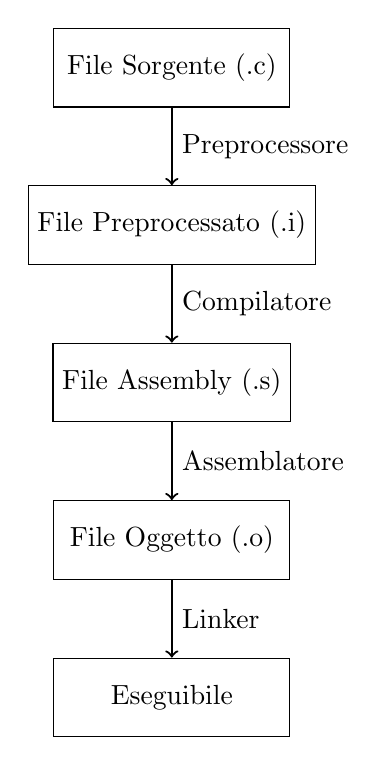
\begin{tikzpicture}[node distance=2cm, auto]
    \node (source) [draw, rectangle, minimum width=3cm, minimum height=1cm] {File Sorgente (.c)};
    \node (preprocessed) [draw, rectangle, minimum width=3cm, minimum height=1cm, below of=source] {File Preprocessato (.i)};
    \node (assembly) [draw, rectangle, minimum width=3cm, minimum height=1cm, below of=preprocessed] {File Assembly (.s)};
    \node (object) [draw, rectangle, minimum width=3cm, minimum height=1cm, below of=assembly] {File Oggetto (.o)};
    \node (executable) [draw, rectangle, minimum width=3cm, minimum height=1cm, below of=object] {Eseguibile};

    \draw[->, thick] (source) -- node {Preprocessore} (preprocessed);
    \draw[->, thick] (preprocessed) -- node {Compilatore} (assembly);
    \draw[->, thick] (assembly) -- node {Assemblatore} (object);
    \draw[->, thick] (object) -- node {Linker} (executable);
\end{tikzpicture}
\caption{Fasi del processo di compilazione}
\end{figure}

\section{Ambiente di Sviluppo}

Per programmare in C hai bisogno di due strumenti fondamentali:

\begin{enumerate}
    \item Un \textbf{editor di testo} o \textbf{IDE} (Integrated Development Environment)
    \item Un \textbf{compilatore C}
\end{enumerate}

\subsection{Installazione del Compilatore GCC}

GCC (GNU Compiler Collection) è il compilatore C più utilizzato, gratuito e open source.

\subsubsection{Su Linux}

\begin{lstlisting}[language=bash, caption={Installazione GCC su Ubuntu/Debian}]
# Aggiorna i repository
sudo apt update

# Installa build-essential (include GCC)
sudo apt install build-essential

# Verifica l'installazione
gcc --version
\end{lstlisting}

\subsubsection{Su macOS}

\begin{lstlisting}[language=bash, caption={Installazione GCC su macOS}]
# Installa Xcode Command Line Tools
xcode-select --install

# Verifica l'installazione
gcc --version
\end{lstlisting}

\subsubsection{Su Windows}

Opzione 1: \textbf{MinGW}
\begin{enumerate}
    \item Scarica MinGW da \url{http://www.mingw.org/}
    \item Installa e aggiungi al PATH
    \item Verifica con \texttt{gcc --version}
\end{enumerate}

Opzione 2: \textbf{WSL} (Windows Subsystem for Linux)
\begin{enumerate}
    \item Abilita WSL nelle impostazioni Windows
    \item Installa una distribuzione Linux (es. Ubuntu)
    \item Segui le istruzioni per Linux
\end{enumerate}

\subsection{Editor e IDE Consigliati}

\begin{description}
    \item[Visual Studio Code] Gratuito, leggero, multipiattaforma. Installa l'estensione "C/C++" di Microsoft.
    \item[Code::Blocks] IDE gratuito specifico per C/C++, semplice e completo.
    \item[Dev-C++] IDE leggero per Windows, ideale per iniziare (ormai obsoleto ma ancora usato in didattica).
    \item[CLion] IDE professionale di JetBrains, gratuito per studenti.
\end{description}

\begin{nota}
Per questo corso consigliamo \textbf{Visual Studio Code} per la sua versatilità, o \textbf{Code::Blocks} per la semplicità d'uso.
\end{nota}

\section{Struttura di un Programma C}

Analizziamo la struttura base di un programma C:

\begin{lstlisting}[caption={Struttura base di un programma C}]
#include <stdio.h>

int main(int argc, char** argv) {
    // Codice del programma
    return 0;
}
\end{lstlisting}

Analizziamo ogni componente:

\subsection{Direttiva \#include}

\begin{lstlisting}
#include <stdio.h>
\end{lstlisting}

\begin{itemize}
    \item \texttt{\#include} è una direttiva del preprocessore
    \item Include il contenuto di un file header
    \item \texttt{<stdio.h>} è la libreria Standard Input/Output
    \item Contiene le dichiarazioni delle funzioni della libreria stdio come \texttt{printf()} e \texttt{scanf()}
\end{itemize}

\subsection{Funzione main()}

\begin{lstlisting}
int main() {
    // ...
    return 0;
}
\end{lstlisting}

\begin{itemize}
    \item \texttt{main()} è la funzione principale del programma
    \item L'esecuzione inizia sempre da \texttt{main()}
    \item \texttt{int} indica che la funzione restituisce un intero
    \item \texttt{return 0} indica che il programma è terminato correttamente
    \item Le parentesi graffe \texttt{\{...\}} delimitano il corpo della funzione
\end{itemize}

\begin{attenzione}
Ogni programma C deve avere una (e una sola) funzione \texttt{main()}. Senza di essa, il programma non può essere eseguito.
\end{attenzione}

\subsection{Commenti}

Il C supporta due tipi di commenti:

\begin{lstlisting}[caption={Tipi di commenti in C}]
// Commento su una singola riga (stile C99)

/* Commento su
   piu' righe
   (stile C89) */

int x = 5;  // Commento a fine riga
\end{lstlisting}

I commenti sono ignorati dal compilatore e servono per documentare il codice.

\section{Il Primo Programma: Hello World}

Scriviamo il tradizionale primo programma:

\begin{lstlisting}[caption={Hello World in C}]
#include <stdio.h>

int main(int argc, char** argv) {
    printf("Hello, World!\n");
    return 0;
}
\end{lstlisting}

\subsection{Analisi del Codice}

\begin{description}
    \item[\texttt{printf()}] La funzione printf() della libreria stdio stampa testo sullo schermo
    \item[\texttt{"Hello, World!"}] La stringa da stampare (racchiusa tra virgolette)
    \item[\texttt{\textbackslash n}] Il carattere speciale: va a capo (newline)
    \item[\texttt{;}] Il punto e virgola: termina ogni istruzione in C
\end{description}

\subsection{Compilazione ed Esecuzione}

\subsubsection{Da Terminale}

\begin{lstlisting}[language=bash, caption={Compilazione ed esecuzione}]
# Compila il programma
gcc hello.c -o hello

# Esegui il programma
./hello           # Su Linux/macOS
hello.exe         # Su Windows
\end{lstlisting}

Opzioni comuni di GCC:
\begin{itemize}
    \item \texttt{-o nome}: specifica il nome del file eseguibile
    \item \texttt{-Wall}: abilita tutti i warning
    \item \texttt{-Wextra}: abilita warning extra
    \item \texttt{-g}: include informazioni di debug
\end{itemize}

\begin{nota}
È buona pratica compilare sempre con \texttt{-Wall -Wextra} per individuare potenziali errori:
\begin{lstlisting}[language=bash]
gcc -Wall -Wextra hello.c -o hello
\end{lstlisting}
\end{nota}

\section{Esempi Guidati}

\subsection{Esempio 1: Stampare Più Righe}

\begin{lstlisting}[caption={Programma con più stampe}]
#include <stdio.h>

int main(int argc, char** argv) {
    printf("Benvenuto nel mondo del C!\n");
    printf("Questo e' il mio primo programma.\n");
    printf("La programmazione e' divertente!\n");
    return 0;
}
\end{lstlisting}

Output:
\begin{verbatim}
Benvenuto nel mondo del C!
Questo e' il mio primo programma.
La programmazione e' divertente!
\end{verbatim}

\subsection{Esempio 2: Caratteri Speciali}

\begin{lstlisting}[caption={Uso di caratteri speciali}]
#include <stdio.h>

int main(int argc, char** argv) {
    printf("Riga 1\n");              // \n va a capo
    printf("Riga 2\tcon tab\n");     // \t inserisce una tabulazione
    printf("Virgolette: \"Ciao\"\n");  // \" stampa le virgolette
    printf("Backslash: \\\n");       // \\ stampa un backslash
    return 0;
}
\end{lstlisting}

Output:
\begin{verbatim}
Riga 1
Riga 2    con tab
Virgolette: "Ciao"
Backslash: \
\end{verbatim}

\subsection{Esempio 3: Stampare Numeri}

\begin{lstlisting}[caption={Stampa di numeri}]
#include <stdio.h>

int main(int argc, char** argv) {
    printf("Il numero e': %d\n", 42);
    printf("Pi greco: %.2f\n", 3.14159);
    printf("Carattere: %c\n", 'A');
    return 0;
}
\end{lstlisting}

Output:
\begin{verbatim}
Il numero e': 42
Pi greco: 3.14
Carattere: A
\end{verbatim}

\begin{nota}
Gli specificatori di formato della funzione printf() (\texttt{\%d}, \texttt{\%f}, \texttt{\%c}) verranno approfonditi nel \autoref{cap:variabili_tipi}.
\end{nota}

\section{Errori Comuni e Debugging}

\subsection{Errore 1: Punto e Virgola Mancante}

\begin{lstlisting}[caption={Errore: punto e virgola mancante}]
#include <stdio.h>

int main() {
    printf("Ciao")   // ERRORE: manca il ;
    return 0;
}
\end{lstlisting}

Messaggio di errore tipico del compilatore:
\begin{verbatim}
error: expected ';' before 'return'
\end{verbatim}

\subsection{Errore 2: Include Mancante}

\begin{lstlisting}[caption={Errore: header mancante}]
// ERRORE: manca #include <stdio.h>

int main() {
    printf("Ciao\n");  // La funzione printf() non e' dichiarata!
    return 0;
}
\end{lstlisting}

\subsection{Errore 3: Parentesi Graffe}

\begin{lstlisting}[caption={Errore: parentesi graffe non bilanciate}]
#include <stdio.h>

int main() {
    printf("Ciao\n");
    return 0;
// ERRORE: manca la } di chiusura
\end{lstlisting}

\begin{errore}
Gli errori di sintassi più comuni per i principianti sono:
\begin{itemize}
    \item Dimenticare il punto e virgola
    \item Non bilanciare le parentesi (tonde, quadre, graffe)
    \item Dimenticare il \texttt{\#include <stdio.h>}
    \item Usare virgolette semplici per stringhe (usare doppie!)
\end{itemize}
\end{errore}

\section{Librerie Standard del C}

Il C fornisce diverse librerie standard utili:

\begin{table}[h]
\centering
\begin{tabular}{|l|l|}
\hline
\textbf{Libreria} & \textbf{Funzionalità} \\
\hline
\texttt{stdio.h} & Input/Output (funzioni printf(), scanf(), fopen(), etc.) \\
\texttt{stdlib.h} & Utility generali (funzioni malloc(), free(), rand(), etc.) \\
\texttt{string.h} & Manipolazione stringhe (funzioni strlen(), strcpy(), etc.) \\
\texttt{math.h} & Funzioni matematiche (funzioni sin(), cos(), sqrt(), etc.) \\
\texttt{time.h} & Gestione data e ora \\
\texttt{ctype.h} & Classificazione caratteri (funzioni isdigit(), isalpha(), etc.) \\
\hline
\end{tabular}
\caption{Principali librerie standard del C}
\end{table}

\section{Best Practices}

\begin{enumerate}
    \item \textbf{Indenta il codice}: Usa 4 spazi o un tab per ogni livello di indentazione
    \item \textbf{Commenta}: Spiega cosa fa il codice, soprattutto le parti complesse
    \item \textbf{Nomi significativi}: Usa nomi descrittivi per variabili e funzioni
    \item \textbf{Una funzionalità per riga}: Evita di mettere troppe operazioni su una singola riga
    \item \textbf{Compila con warning}: Usa sempre \texttt{-Wall -Wextra}
\end{enumerate}

\section{Esercizi}

\subsection{Livello Base}

\begin{enumerate}
    \item Scrivi un programma che stampa il tuo nome e cognome su righe separate.
    \item Crea un programma che stampa un rettangolo di asterischi (5 righe x 10 colonne).
    \item Scrivi un programma che stampa la scritta "C Programming" usando caratteri ASCII art.
\end{enumerate}

\subsection{Livello Intermedio}

\begin{enumerate}
    \item Scrivi un programma che stampa i primi 10 numeri (da 1 a 10) usando 10 printf separate.
    \item Crea un programma che stampa una piccola storia su più righe, usando tabulazioni per l'indentazione dei dialoghi.
    \item Scrivi un programma che stampa una tabella formattata con informazioni personali (nome, età, città).
\end{enumerate}

\subsection{Livello Avanzato}

\begin{enumerate}
    \item Ricerca online come usare i codici ANSI per colorare il testo nel terminale e scrivi un programma che stampa testo colorato.
    \item Scrivi un programma che stampa un menu di un'applicazione (simulato) con bordi e formattazione.
\end{enumerate}

\section{Riepilogo}

In questo capitolo abbiamo imparato:

\begin{itemize}
    \item La storia e le caratteristiche del linguaggio C
    \item La differenza tra compilazione e interpretazione
    \item Come installare e configurare l'ambiente di sviluppo
    \item La struttura base di un programma C
    \item Come scrivere, compilare ed eseguire il primo programma
    \item Gli errori comuni e come risolverli
    \item Le principali librerie standard
\end{itemize}

\section{Approfondimenti}

Per approfondire gli argomenti di questo capitolo:

\begin{itemize}
    \item \textbf{Libro}: "The C Programming Language" - Kernighan \& Ritchie (capitolo 1)
    \item \textbf{Online}: C Tutorial su Learn-C.org
    \item \textbf{Video}: Playlist "C Programming for Beginners" su YouTube
    \item \textbf{Documentazione}: GCC Manual (\url{https://gcc.gnu.org/onlinedocs/})
\end{itemize}

Nel \autoref{cap:variabili_tipi} inizieremo a lavorare con variabili e tipi di dati, rendendo i nostri programmi interattivi!
